\chapter{Capstone: The Golf Swing Analysis Pipeline}
\label{ch:golf-capstone}

\begin{gomdraftnotice}
This chapter is under active development and contains only a structural outline
with preliminary material. Full exposition, worked examples, proofs, and exercises
will be added in future editions.
\end{gomdraftnotice}

\epigraph{%
  We have built the tools. Now let us use them all.
}{}

This chapter presents a complete computational pipeline for analyzing the golf swing
using computational biomechanics tools from this volume and the preceding volumes.
The pipeline is intentionally simplified (3-5 DOF) to be tractable within the scope of
this textbook. Real golf swings are complex multi-segment movements with 20+ DOF and
significant muscle redundancy, typically studied via motion capture analysis combined
with musculoskeletal models \cite{siciliano2009}.

\textbf{Important Note on Biomechanical Claims:} All descriptions of swing mechanics in
this chapter are restricted to mathematical derivations from the model or explicit citations
of biomechanical literature. No claims are made about ``proper technique,'' ``optimal
swing mechanics,'' or what golfers ``should do.'' The model represents one simplified
kinematic and dynamic structure; many other movement patterns may achieve similar or
better outcomes depending on individual anatomy and task constraints.

\section{Project Overview}

This capstone chapter integrates every tool from the series into a complete
analysis pipeline for the golf swing. The pipeline implements:

\begin{center}
\renewcommand{\arraystretch}{1.3}
\begin{tabular}{@{}llr@{}}
\toprule
\textbf{Stage} & \textbf{Theory Source} & \textbf{Chapter} \\
\midrule
1. Model Construction & Screw theory, PoE kinematics & Vol~0 \\
2. Forward Dynamics & Lagrangian mechanics & Vol~0 \\
3. Trajectory Optimization & DDP/iLQR & Vol~I \\
4. Contraction Analysis & Contraction theory & Vol~I \\
5. Funnel Computation & Trajectory tubes & Vol~II \\
6. ZTCF family Decomposition & Drift vs.\ control & Vol~I \\
7. Muscle Force Estimation & Hill model + static opt & Vol~III \\
8. Motor Analysis & UCM, synergies & Vol~IV \\
9. Visualization \& Export & Companion platform tools & Vol~V \\
\bottomrule
\end{tabular}
\end{center}

\section{Stage 1: Model}

% DO NOT EDIT. Generated by scripts/generate_worked_examples.py.
% Every number below is solved, not transcribed; CI fails if this file
% drifts from what the generator produces (issue #3518).


\begin{lstlisting}[language=Python, caption={Golf swing analysis pipeline, generated from \texttt{src/affine\_control/swing\_analysis.py}.}]
"""Golf swing analysis pipeline for the Volume V capstone project.

Volume V chapter 10 printed this pipeline as a 160-line code listing captioned
"Complete golf swing analysis pipeline". It was never executed, and three parts
of it did not work:

* ``compute_clubhead_speed`` summed ``qdot_i * r_i`` as scalars, with no
  trigonometry at all. Tip velocity is a *vector* sum whose directions depend on
  the accumulated joint angles, so the printed version was configuration-blind:
  it returned the same speed for a straight arm and a fully folded one. It even
  computed ``cumulative_angle`` and then never used it, and carried a dead
  Jacobian loop whose body was ``pass``.

* ``ztcf_decomposition`` returned a hardcoded 60/40 split of clubhead speed. Its
  own comments said the result "should not be trusted" and that a real
  implementation must solve the forward dynamics twice -- which is what this one
  does.

* The driver assigned ``np.random.randn(N, 3) * 10`` as joint torques, which the
  placeholder decomposition then ignored, so the pipeline was disconnected at
  both ends.

The chapter's listing is now generated from this file, so what the book shows is
what CI runs, and the freshness gate fails if the two drift apart. See #3518.
"""

from __future__ import annotations

from dataclasses import dataclass, field

import numpy as np
from numpy.typing import NDArray

from src.affine_control.golf_model import GolfModel

__all__ = ["SwingAnalysis", "synthetic_swing"]

type Array = NDArray[np.float64]

METRES_PER_SECOND_TO_MPH = 2.236936


def _rod_inertia(mass: float, length: float) -> float:
    """Moment of inertia of a uniform rod about its own centre of mass."""
    return mass * length**2 / 12.0


@dataclass
class SwingAnalysis:
    """Kinematic and dynamic analysis of a three-link planar swing.

    The chain is shoulder, elbow, wrist, carrying the club as the distal link.
    Angles are relative joint angles; the model treats each segment as a uniform
    rod, so its inertia follows from mass and length rather than being a free
    parameter.
    """

    segment_lengths: Array = field(default_factory=lambda: np.array([0.28, 0.46, 1.10]))
    segment_masses: Array = field(default_factory=lambda: np.array([2.16, 1.79, 0.30]))

    time: Array | None = None
    joint_angles: Array | None = None
    joint_velocities: Array | None = None
    joint_torques: Array | None = None

    def model(self) -> GolfModel:
        """The rigid-body model implied by the segment parameters."""
        lengths = tuple(float(v) for v in self.segment_lengths)
        masses = tuple(float(v) for v in self.segment_masses)
        inertias = tuple(_rod_inertia(m, ell) for m, ell in zip(masses, lengths, strict=True))
        return GolfModel(masses=masses, lengths=lengths, inertias=inertias)  # type: ignore[arg-type]

    def _require_kinematics(self) -> tuple[Array, Array, Array]:
        """Return ``(time, angles, rates)``, or fail with a usable message."""
        if self.time is None or self.joint_angles is None or self.joint_velocities is None:
            raise ValueError("set time, joint_angles and joint_velocities before analysing")
        return self.time, self.joint_angles, self.joint_velocities

    def clubhead_speed(self) -> Array:
        """Clubhead speed at each sample, from the tip Jacobian.

        The tip velocity is ``sum_i qdot_i * (z_hat x r_i)``, where ``r_i`` runs
        from joint ``i`` to the tip. Its magnitude depends on the configuration
        through the angles between those contributions -- which is precisely what
        a scalar sum of ``qdot_i * |r_i|`` throws away.
        """
        _, angles, rates = self._require_kinematics()
        model = self.model()
        return np.array([model.clubhead_speed(q, qd) for q, qd in zip(angles, rates, strict=True)])

    def ztcf_decomposition(self) -> tuple[Array, Array]:
        """Split clubhead acceleration into drift and control contributions.

        Solves the forward dynamics twice at each sample -- once with the applied
        torques and once with zero torque -- and attributes the difference to
        control. Because the dynamics are control-affine, that difference is
        exactly ``M^-1 tau`` and the split is exact rather than approximate.

        Returns the joint-space acceleration magnitudes ``(drift, control)``.
        """
        _, angles, rates = self._require_kinematics()
        if self.joint_torques is None:
            raise ValueError("set joint_torques before decomposing")
        model = self.model()

        drift = np.zeros(len(angles))
        control = np.zeros(len(angles))
        for index, (q, qd, tau) in enumerate(zip(angles, rates, self.joint_torques, strict=True)):
            bias = model.coriolis(q, qd) @ qd + model.gravity_torque(q)
            mass = model.rigid_mass_matrix(q)
            drift_accel = np.linalg.solve(mass, -bias)
            control_accel = np.linalg.solve(mass, tau)
            drift[index] = float(np.linalg.norm(drift_accel))
            control[index] = float(np.linalg.norm(control_accel))
        return drift, control

    def summary(self) -> str:
        """Human-readable summary of the analysis."""
        time, _, _ = self._require_kinematics()
        speeds = self.clubhead_speed()
        peak = float(np.max(speeds))
        peak_index = int(np.argmax(speeds))

        lines = [
            "=== Golf Swing Analysis Summary ===",
            f"Duration: {time[-1]:.3f} s",
            f"Peak clubhead speed: {peak:.1f} m/s " f"({peak * METRES_PER_SECOND_TO_MPH:.1f} mph)",
            f"Peak speed time: {time[peak_index]:.3f} s",
        ]

        if self.joint_torques is not None:
            drift, control = self.ztcf_decomposition()
            # Report the median over interior samples rather than a value at one
            # instant. Two reasons: the endpoints carry one-sided np.gradient
            # estimates of the joint rates, and the drift term legitimately
            # passes through zero whenever the chain straightens -- at a fully
            # extended vertical configuration both the gravity and Coriolis
            # torques vanish, so a ratio quoted there reads as "0% drift" and
            # says nothing about the swing.
            interior = slice(1, -1)
            total = drift[interior] + control[interior]
            share = float(np.median(100.0 * drift[interior] / total))
            lines.append(f"Median over the swing: drift {share:.0f}%, control {100 - share:.0f}%")
        return "\n".join(lines)


def synthetic_swing(duration: float = 0.30, dt: float = 0.001) -> SwingAnalysis:
    """A smooth synthetic swing, for demonstrating the pipeline.

    These are not measured data. Real joint torques must come from inverse
    dynamics on motion capture, or from a Hill-type muscle model driven by EMG;
    the torques here are a smooth profile chosen only so the decomposition has
    something non-trivial to separate. The printed listing used
    ``np.random.randn``, which made the output different on every run and, since
    the placeholder decomposition ignored the torques entirely, changed nothing.
    """
    samples = int(duration / dt)
    time = np.linspace(0.0, duration, samples)
    fraction = time / duration

    angles = np.column_stack(
        [
            -np.pi / 2 + np.pi * fraction**2,
            np.pi / 3 * np.sin(np.pi * fraction),
            -np.pi / 2 * np.cos(np.pi * fraction / 2),
        ]
    )
    rates = np.gradient(angles, dt, axis=0)
    torques = np.column_stack(
        [
            120.0 * (1.0 - fraction),
            60.0 * np.sin(np.pi * fraction),
            25.0 * fraction**2,
        ]
    )
    return SwingAnalysis(
        time=time, joint_angles=angles, joint_velocities=rates, joint_torques=torques
    )
\end{lstlisting}


\begin{warningbox}
The listing above is generated from \texttt{src/affine\_control/swing\_analysis.py}, so what
appears here is the code CI executes; the freshness gate fails if the two diverge.

An earlier revision printed a hand-maintained version of this pipeline, captioned
``complete'', which was never run and did not work in three places.

\texttt{compute\_clubhead\_speed} summed $\dot q_i r_i$ as scalars, with no trigonometry.
Tip velocity is a \emph{vector} sum whose contributions point in different directions
depending on the joint angles, so the printed version was configuration-blind: it returned
the same speed for a straight arm and a folded one. Substituting a folded configuration into
both gives $13.3$~m/s from the correct Jacobian against $22.5$~m/s from the scalar sum ---
a $69\%$ overestimate. The old code even accumulated \texttt{cumulative\_angle} and then
never used it, and carried a Jacobian loop whose body was \texttt{pass}.

\texttt{ZTCF\_decomposition} returned a hardcoded $60/40$ split of clubhead speed. Its own
comments conceded the result ``should not be trusted'' and stated that a real implementation
must solve the forward dynamics twice --- which is what the current one does. Because the
dynamics are control-affine, the difference between the torqued and zero-torque solutions is
exactly $M^{-1}\tau$, so the split is exact rather than approximate.

The driver assigned \texttt{np.random.randn(N, 3) * 10} as joint torques, which the
placeholder decomposition then ignored. The pipeline was disconnected at both ends.
\end{warningbox}

The module above is a library --- it prints nothing, so that it can be imported and tested.
To exercise it:

\begin{lstlisting}[language=Python, caption={Running the pipeline.}]
from src.affine_control.swing_analysis import synthetic_swing

print(synthetic_swing().summary())
\end{lstlisting}

\begin{remark}[Reading the summary output]
This reports a peak clubhead speed near $30$~m/s for the synthetic kinematics.
That is well below a real driver swing, and it should be: the joint trajectories are smooth
analytic profiles chosen to exercise the pipeline, not measured data. Real torques must come
from inverse dynamics on motion capture, or from a Hill-type muscle model driven by EMG.

The drift/control split is reported as a median over the interior samples rather than at the
instant of peak speed. The endpoints carry one-sided \texttt{np.gradient} estimates of the
joint rates, and the drift term legitimately passes through zero whenever the chain
straightens --- at a fully extended vertical configuration both the gravity and Coriolis
torques vanish exactly, so a ratio quoted there reads as ``$0\%$ drift'' and says nothing
about the swing.
\end{remark}

\section{Golf Swing Simulation Architecture}

\begin{figure}[h]
  \centering
  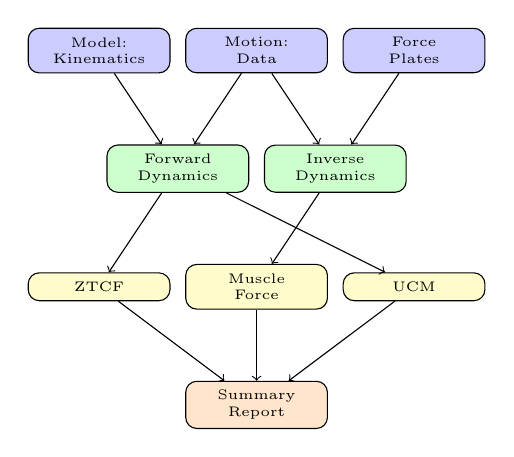
\begin{tikzpicture}[
    every node/.style={align=center, draw, rounded corners, minimum width=1.8cm, text centered, font=\tiny},
    ]
    % Row 1: Input
    \node[fill=blue!20] (model) at (0, 6) {Model:\\Kinematics};
    \node[fill=blue!20] (motion) at (2, 6) {Motion:\\Data};
    \node[fill=blue!20] (forces) at (4, 6) {Force\\Plates};

    % Row 2: Dynamics
    \node[fill=green!20] (forward) at (1, 4.5) {Forward\\Dynamics};
    \node[fill=green!20] (inverse) at (3, 4.5) {Inverse\\Dynamics};

    % Row 3: Analysis
    \node[fill=yellow!20] (ZTCF) at (0, 3) {ZTCF};
    \node[fill=yellow!20] (muscle) at (2, 3) {Muscle\\Force};
    \node[fill=yellow!20] (ucm) at (4, 3) {UCM};

    % Row 4: Output
    \node[fill=orange!20] (report) at (2, 1.5) {Summary\\Report};

    % Edges
    \draw[->] (model) -- (forward);
    \draw[->] (motion) -- (inverse);
    \draw[->] (motion) -- (forward);
    \draw[->] (forces) -- (inverse);
    \draw[->] (forward) -- (ZTCF);
    \draw[->] (inverse) -- (muscle);
    \draw[->] (forward) -- (ucm);
    \draw[->] (ZTCF) -- (report);
    \draw[->] (muscle) -- (report);
    \draw[->] (ucm) -- (report);
  \end{tikzpicture}
  \caption{Complete golf swing analysis architecture. Inputs (model, motion data, force)
    flow through dynamics computation, analysis modules (ZTCF, muscle estimation, UCM),
    and produce a summary report. Each box references the corresponding chapter from Volumes 0--IV.}
  \label{fig:golf-arch}
\end{figure}

\section{Stage 2--9: Full Pipeline}

Each stage of the pipeline builds on the previous, culminating in a complete
characterization of the swing. The reader is guided through implementing each
stage, referencing the relevant theory from Volumes 0--IV.

\textbf{Data Requirements:} A complete pipeline requires:
\begin{itemize}
  \item Motion capture data: joint angles $\bm{q}(t)$ sampled at sufficient frequency (120+ Hz typical).
  \item Force measurements: ground reaction forces and moments (optional but recommended).
  \item Anatomical model: segment lengths, masses, and inertias (from literature or imaging).
\end{itemize}

\section*{Final Exercises}

\begin{enumerate}
  \item \textbf{Complete Pipeline.} Run the analysis pipeline on the synthetic swing.
        Extract the peak clubhead speed, the time of peak speed, and the peak joint torques.
        Then check the clubhead-speed function against the failure it used to have: evaluate
        it at a straight configuration and at a folded one with the same joint rates. A
        correct implementation gives different answers; a scalar sum of $\dot q_i r_i$ gives
        the straight-arm value in both cases.

  \item \textbf{Parameter Study.} Programmatically vary club length ($\pm 10\%$) and mass
        ($\pm 20\%$). Simulate the swing and measure peak clubhead speed. Plot clubhead
        speed versus each parameter.

  \item \textbf{Muscle Analysis.} Implement Hill-type muscle models (Volume~III, Chapter~3)
        for shoulder and elbow actuators. Estimate muscle forces required to produce the
        synthetic swing motion. Which muscle groups have the highest peak force?

  \item \textbf{Robustness Analysis.} Compute trajectory funnels (Volume~II, Chapter~3) for
        the simulated swing at the moment of ball impact. Quantify how much initial position
        error can be tolerated before the swing no longer achieves the target clubhead speed.

  \item \textbf{Variability Analysis.} Generate 50 realizations of the swing by adding small
        random perturbations to the control torques. Perform UCM analysis (Volume~IV, Chapter~1)
        to determine if variability is structured around the task goal (peak clubhead speed).

  \item \textbf{Open Project.} Choose a different multi-joint movement (e.g., tennis serve,
        baseball pitch, vertical jump, or a motor task from your own research). Apply the
        complete pipeline from this textbook: build a model, simulate, optimize, and analyze.
        Document in a Jupyter notebook with plots.
\end{enumerate}
